\documentclass[a4paper]{article}
\usepackage[utf8]{inputenc}
\usepackage{amsmath}
\usepackage{siunitx}
\usepackage[ngerman]{babel}
\usepackage{pgfplots}
\usepackage{hyperref}
\usepackage{pgfplotstable}
\usepackage[section]{placeins}
\usepackage{enumitem}
\usepackage{float}
\usepackage{booktabs}
\usepackage{subcaption}

\pgfplotsset{compat=1.15}

% Full Reference, produces: "Abbildung 3: Schaltplan"
\newcommand*{\fullref}[1]{\hyperref[{#1}]{\autoref*{#1}: \nameref*{#1}}}

\title{GPET\\ Auswertung Versuch 5\\ Gruppe 1}

\author{Jonas Otto\\ \href{mailto:jonas@jonasotto.com}{jonas@jonasotto.com} 
   \and Luca Krüger \\ \href{mailto:luca.krueger@uni-ulm.de}{luca.krueger@uni-ulm.de} }
\date{15. Mai 2018}

\begin{document}
    
\maketitle
\newpage
\section{Versuchsauswertung}
\subsection{Vorbemerkung}
In diesem Praktikum gab es massive Probleme mit der Messgenauigkeit beim Versuchsaufbau. Die Signale an an beiden Eingängen des Oszilloskopes wurden von einem starken Rauschen überlagert. Dadurch war es nicht möglich einen geeigneten Trigger einzustellen, um ein stehendes Signal am Oszilloskop bekommen. Die Autoscale-Funktion am Oszilloskop hat ebenfalls nicht funktioniert. Es wurde viel Zeit aufgewendet, um mögliche Fehlerquellen auszuschließen.
Letztendlich wurde das Oszilloskop als Fehlerquelle identifiziert. Ein anderes Oszilloskop stand nicht zur Verfügung.
Fehlerhafte Messwerte gibt es nun vorallem bei den Amplitudenmessungen und bei Messungen mit der Matlab-Gui. 
Die automatische Measure-Funktion hat Spitzen, die durch das Rauschen verursacht wurden fälschlicherweise als Amplitude aufgefasst. Dadurch sind stark vom erwarteten Wert abweichende Messwerte zu Amplituden und den daraus resultierendem Spannungsverhältnis zu erklären.
Deshalb wurden teilweise die Messungen  mit Hilfe der Cursor durchgeführt. Dies war aber aufgrund der hohen Anzahl vorgegebener Messpunkte nicht bei jeder Messung möglich.
Im folgenden wird nicht jeder fehlerhafte Messwert explizit erläutert, sondern hiermit auf die vorhergehende Erklärung verweisen.
\subsection{Spannungsübersetzung beim unbelasteten Transformator} 
\label{subsec:Versuch1-unbelastet}

Mit der Schaltung aus Abbildung \ref{fig:1-versuchsaufbau} wurden verschiedene Übersetzungsverhältnisse des unbelasteten Transformators betrachtet.
Die Spannungsquelle $\underline{U}_\textit{ein}$ erzeugt ein Sinussignal der Frequenz $f=500\si{Hz}$ mit Peak-zu-Peak Spannung $V_\textit{pp}=1\si{V}$.
Die Messwerte zur Primärspannung $U_1$, Sekundärspannung $U_2$ und das daraus resultierende Spannungsverhältnis $\frac{U_2}{U_1}$ werden in \fullref{tab:1-messtab} aufgeführt.\

Die Messwerte bestätigen die Abhängigkeit $\frac{U_2}{U_1}=\frac{N_2}{N_1}$ zwischen dem Spannungsverhältnis $\frac{U_2}{U_1}$ und dem Windungsverhältnis $\frac{N_2}{N_1}$. Durch Streuflüsse entstehen außerdem kleine Verluste bei der Spannungsübertragung. Dadurch fällt das Übertragungsverhältnis tendenziell geringer aus.


\begin{figure}[H]
    \centering
    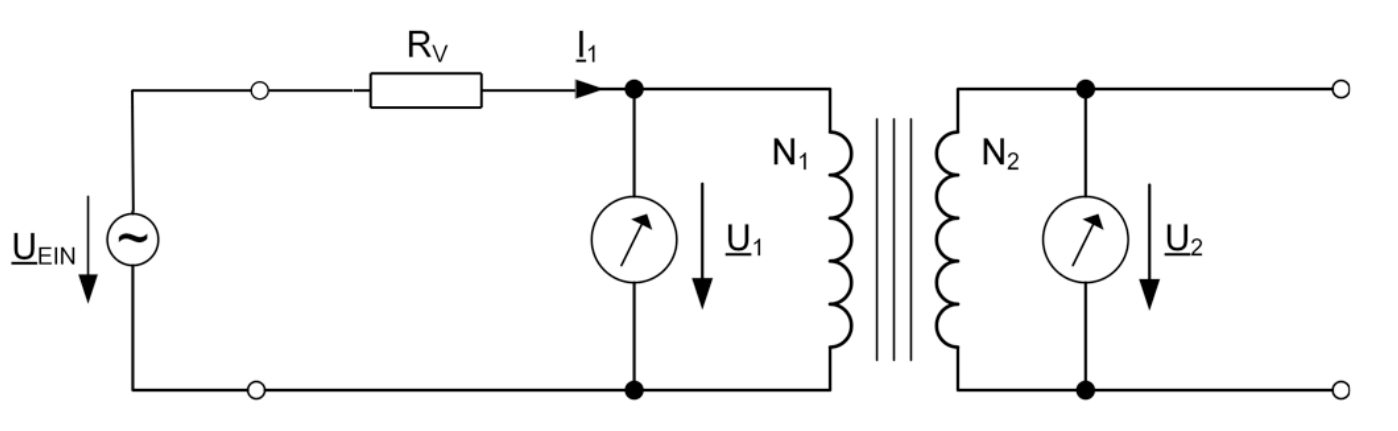
\includegraphics[width=0.8\textwidth]{versuchsaufbau-1.png}
    \caption[Schaltplan]{Versuchsaufbau zu Versuch: \nameref{subsec:Versuch1-unbelastet}}
    \label{fig:1-versuchsaufbau}
\end{figure}

\begin{table}[H]
    \centering
    \begin{tabular}{S S S S S}
         \toprule
        {$N_1$} & {$N_2$} & {$U_1 [\textbf{V}]$} & {$U_2 [\textbf{V}]$} & {$U_2/U_1$} \\ 
        \midrule
        250 & 500 & 0.63 & 0.8 & 1.27\\
        500 & 500 & 1.01 & 0.78  & 0.77\\
        1000 & 500 & 1.15 & 0.56 & 0.49\\
        1000 & 250 & 1.11 & 0.32 & 0.29\\
        \bottomrule
    \end{tabular}
    \caption{Messtabelle zu Versuch 1}
    \label{tab:1-messtab}
\end{table}

\subsection{Der belastete Transformator}
\label{subsec:Versuch2-belastet}
In diesem Versuch wurde der Einfluss verschiedener Lastwiderstände auf die Spannungstransformation eines belasteten Transformators betrachtet.
Die Schaltskizze dazu ist in Abblidung \ref{fig:2-versuchsaufbau} zu sehen. Die Spannungsquelle $\underline{U}_\textit{ein}$ ist wie in Versuch \ref{subsec:Versuch1-unbelastet} \glqq \nameref{subsec:Versuch1-unbelastet}\grqq ein Frequenzgenerator mit eingestelltem Sinussignal der Frequenz $f=500\si{Hz}$ und Peak-zu-Peak Spannung $V_\textit{pp}=1\si{V}$. Der Widerstand $R_v$ beträgt $100\si{\ohm}$
Der Versuch wurde mit zwei verschiedenen Windungsverhältnissen $n_1=\frac{N_1}{N_2}=\frac{500}{500}$ und $n_2=\frac{250}{500}$ durchgeführt.
Dabei wurden jeweils zehn unterschiedliche Lastwiderstände $R_L$ im Bereich von $100\si{\ohm}$ und $1000\si{\ohm}$ eingestellt und zu jeder Variation die Primärspannung $\underline{U}_1$, Sekundärspannung $\underline{U}_2$ und das daraus resultierende Spannungsverhältnis $\frac{\underline{U}_2}{\underline{U}_1}$ gemessen. Die Werte dieser Messungen sind in Tabelle \ref{tab:2-messtab} aufgeführt. 

\begin{figure}[H]
    \centering
    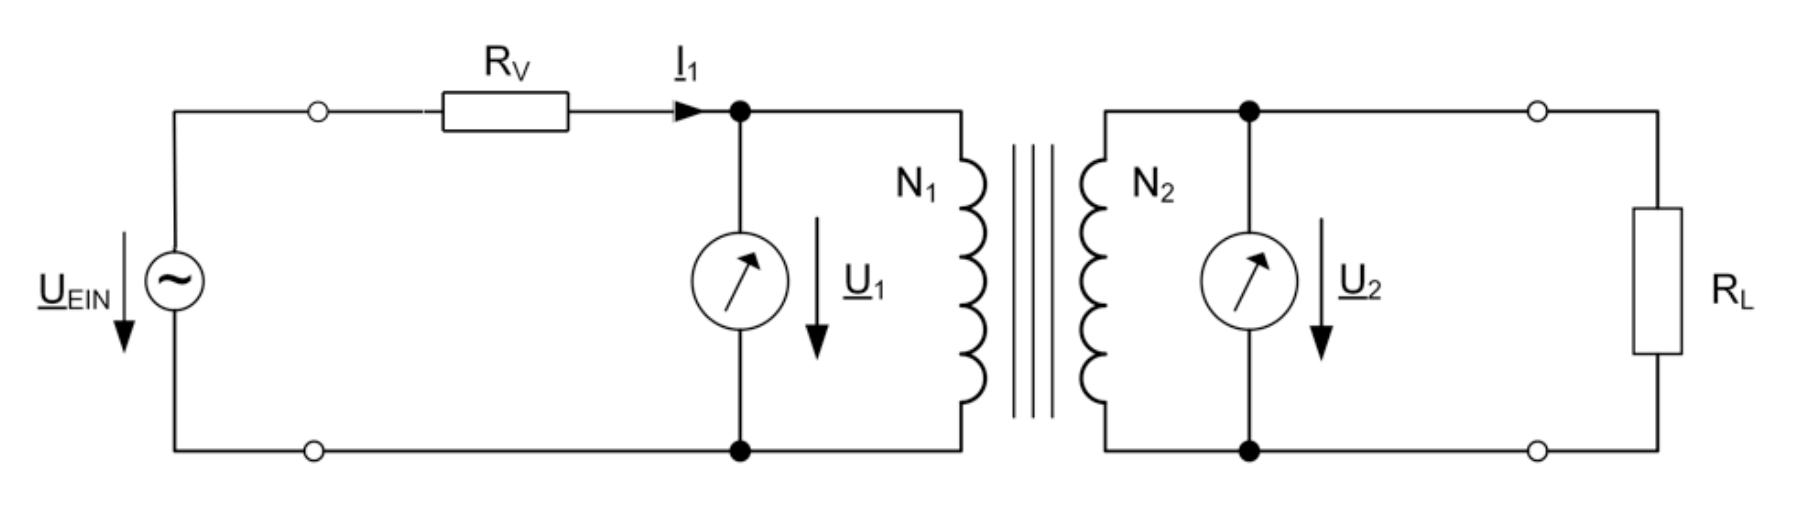
\includegraphics[width=0.8\textwidth]{versuchsaufbau-2.png}
    \caption{Versuchsaufbau zu Versuch: \nameref{subsec:Versuch2-belastet}}
    \label{fig:2-versuchsaufbau}
\end{figure}

\begin{table}[H]
    \centering
    \begin{tabular}{c c *{10}{S[table-format=2.2, tight-spacing=true] }}
         \toprule
         & {$R_L [\si{\ohm}]$} & {100} & {150} & {200} & {250} & {300} & {350} & {400} & {600} & {800} & {1000} \\ 
        \midrule
         & {$U_1[\text{V}]$}                & 0.84 & 0.86 & 0.88 & 0.96 & 0.90 & 0.84 & 0.84 & 1.10 & 0.84 & 0.91\\
        {$500:500$} & {$U_2[\text{V}]$}     & 0.25 & 0.33 & 0.53 & 0.43 & 0.46 & 0.78 & 0.82 & 0.76 & 0.78 & 0.80\\
         & {$U_2/U_1$}                      & 0.29 & 0.38 & 0.60 & 0.45 & 0.51 & 1.03 & 0.97 & 0.69 & 0.93 & 0.87 \\
        \midrule
         & {$U_1[\text{V}]$}                & 0.23 & 0.28 & 0.29 & 0.31 & 0.32 & 0.33 & 0.36 & 0.38 & 0.40 & 0.41\\
        {$250:500$} & {$U_2[\text{V}]$}     & 0.19 & 0.28 & 0.34 & 0.40 & 0.43 & 0.47 & 0.49 & 0.55 & 0.60 & 0.62\\
         & {$U_2/U_1$} 
         & 0.82 & 1 &1.17 & 1.29 & 1.34 & 1.42 & 1.36 & 1.44 & 1.5 & 1.51 \\
        \bottomrule
    \end{tabular}
    \caption{Messtabelle zu Versuch: \nameref{subsec:Versuch2-belastet}}
    \label{tab:2-messtab}
\end{table}

Aus den Messwerten ist ersichtlich, dass die Abweichung der Spannungsverhältnisse zum erwarteten Wert (unbelastet) mit zunehmendem Lastwiderstand geringer wird. Bei großer Last gleicht sich die Spannungsübertragung der eines Leerlaufes an. Mit einem kleinen Lastwiderstand  fließt ein größerer Strom auf der Sekundärseite. Das wird auf der Primärseite kompensiert und das Spannungsverhältnis bricht ein.

\subsection{Kopplungsgrad}
\label{subsec:Versuch3-Kopplungsgrad}

\begin{figure}[H]
    \centering
    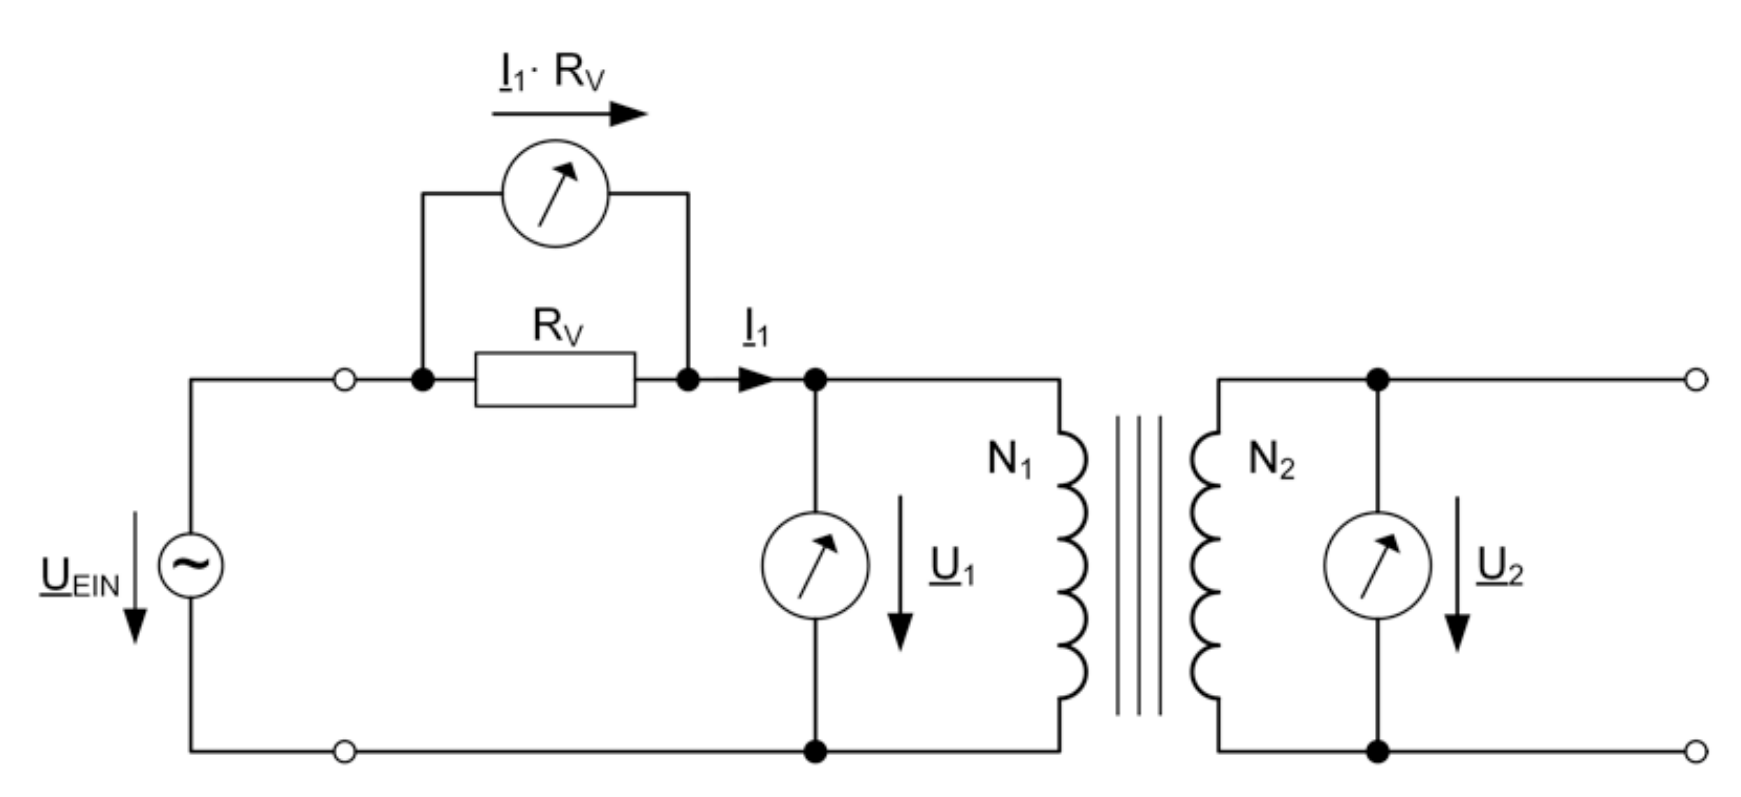
\includegraphics[width=0.8\textwidth]{versuchsaufbau-3-kopplungsgrad.png}
    \caption[Schaltplan]{Versuchsaufbau zu Versuch: \nameref{subsec:Versuch3-Kopplungsgrad}}
    \label{fig:3-versuchsaufbau-kopplungsgrad}
\end{figure}

\begin{figure}[H]
    \centering
    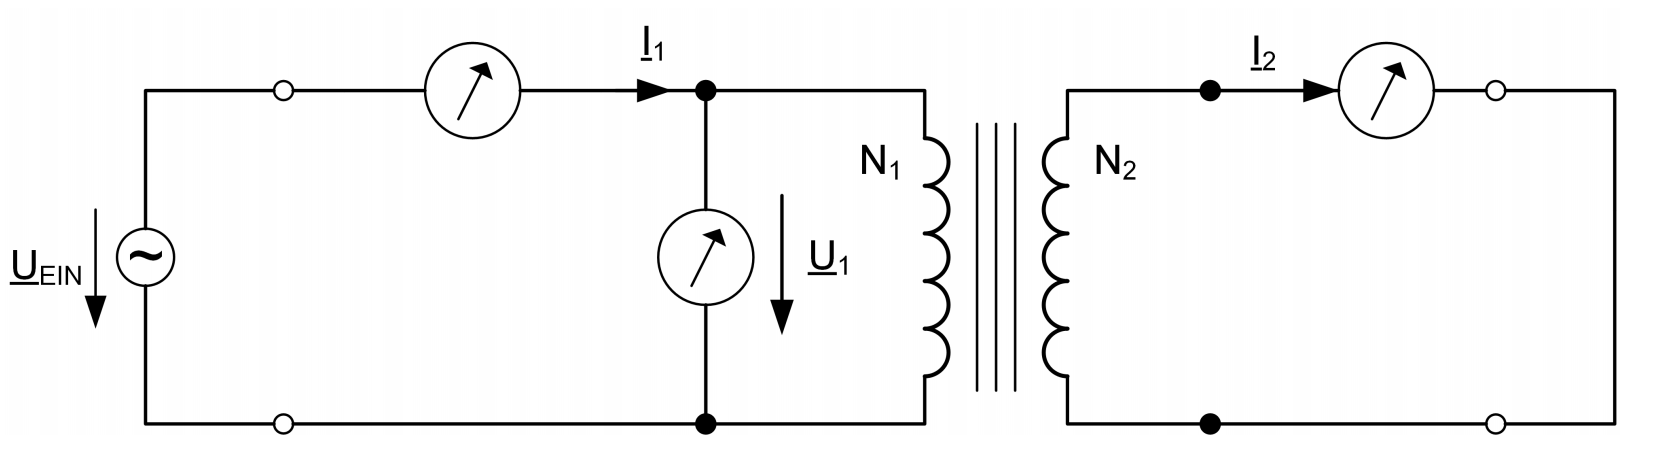
\includegraphics[width=0.8\textwidth]{versuchsaufbau-3-kurzschluss.png}
    \caption[Schaltplan]{Versuchsaufbau zu Versuch: \nameref{subsec:Versuch3-Kopplungsgrad}}
    \label{fig:3-versuchsaufbau-kurzschluss}
\end{figure}

\paragraph{}
Für $f_1=500\si{Hz}$:

$$I_1=\frac{U_R}{100\si{\ohm}}=\frac{248\si{mV}}{100\si{\ohm}}=2.48\si{mA}$$
$$L_1=\frac{U_1}{\omega I_1}=\frac{855\si{mV}}{2 \pi 500\si{Hz} 0.88\si{mA}}=109.7\si{mH}$$
$$M=\frac{U_2}{\omega I_1}=\frac{622\si{mV}}{2 \pi \cdot 500\si{Hz} \cdot 2.48\si{mA}}=79.8\si{mH}$$
$$L_2=\frac{M I_1}{I_2}=\frac{79.8\si{mH} \cdot 4.2\si{mA}}{3.3\si{mA}}=101.5\si{mH}$$

$$k=\frac{M}{\sqrt{L_1\cdot L_2}}=\frac{79.8\si{mH}}{\sqrt{109.7\si{mH} \cdot 101.5\si{mH}}} = 0.756$$


%für l2
%I_1=4,2mA
%I_2=3,3mA

Für $f_2=5\si{kHz}$:
%U_1pp=970mV
%U_2pp=705mV
%U_Reff=8.5mV

%für l2
%I_1=0,46mA
%I_2=0,32mA

$$I_1=\frac{U_R}{100\si{\ohm}}=\frac{24\si{mV}}{100\si{\ohm}}=0.24\si{mA}$$
$$L_1=\frac{U_1}{\omega I_1}=\frac{970\si{mV}}{2 \pi 5\si{kHz} 0.24\si{mA}}=129\si{mH}$$
$$M=\frac{U_2}{\omega I_1}=\frac{705\si{mV}}{2 \pi \cdot 5\si{kHz} \cdot 0.24\si{mA}}=93\si{mH}$$
$$L_2=\frac{M I_1}{I_2}=\frac{93\si{mH} \cdot 0.46\si{mA}}{0.32\si{mA}}=134\si{mH}$$

$$k=\frac{M}{\sqrt{L_1\cdot L_2}}=\frac{93\si{mH}}{\sqrt{129\si{mH} \cdot 134\si{mH}}} = 0.7$$

Die Werte für $L_1$, $L_2$, $M$ und damit auch für den Kopplungsgrad sind offensichtlich frequenzabhängig.
Die Streuinduktivitäten $L_1$ und $L_2$ sind bei der Frequenz $f_2$ ca. $30\%$ höher als bei $f_1$. Die Übertragung ist bei niedrigerer Frequenz also effizienter und der Kopplungsgrad damit auch größer.
\subsection{Frequenzabhängiges Übertragungsverhalten und Phasenschiebung unter Last}
\label{subsec:Versuch4-Frequenz}

Wie in der Bode-Diagrammen zu erkennen ist, ist die $3\si{dB}$-Grenzfrequenz abhängig von der Last $R_L$. Das Verhalten des Transformators gleicht dem eines Tiefpasses. Bei höherem Lastwiderstand $R_L$ ist die Grenzfrequenz höher. Das bestätigt auch unsere vorbereiteten Berechnungen, wonach das Übertragungsverhältnis $H_\textit{trafo}=\frac{R_L}{R_L+j\omega L_\textit{S2}}*\frac{N_2}{N_1}*\frac{L_{h1}}{L_{S1}}$ beträgt. Die Grenzfrequenz ist dann insofern vom Lastwiderstand abhängig, als dass gilt $H_\textit{trafo}(\omega_g)=\frac{R_L}{R_L+j\omega_g L_\textit{S2}}*\frac{N_2}{N_1}*\frac{L_{h1}}{L_{S1}}=\frac{1}{\sqrt{2}}$.

\begin{figure}[H]
    \centering
    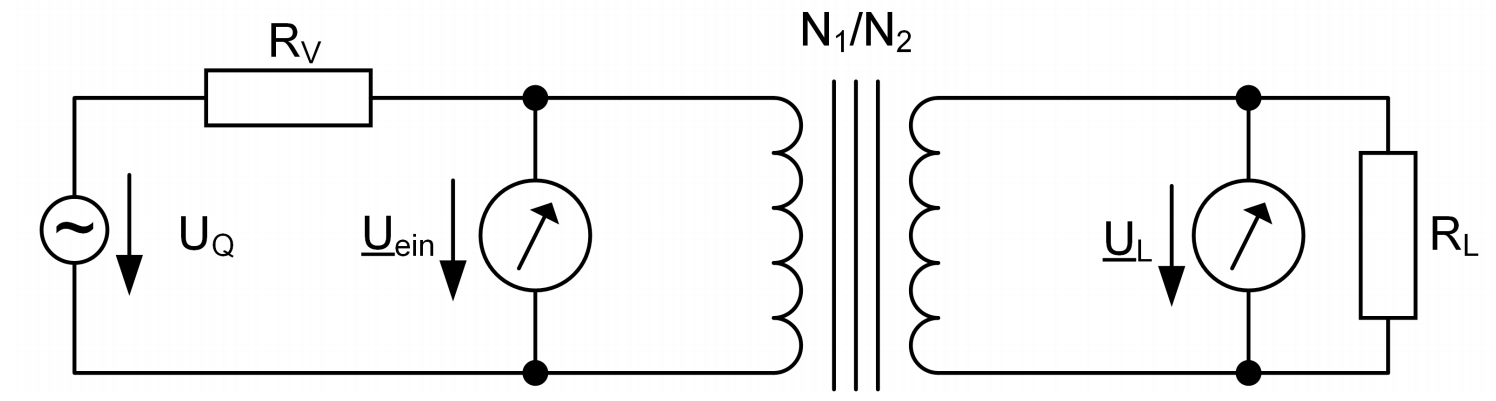
\includegraphics[width=0.8\textwidth]{versuch4/versuchsaufbau-4.png}
    \caption[Schaltplan]{Versuchsaufbau zu Versuch: \nameref{subsec:Versuch4-Frequenz}}
    \label{fig:4-versuchsaufbau}
\end{figure}

\begin{figure}[H]
        \centering
        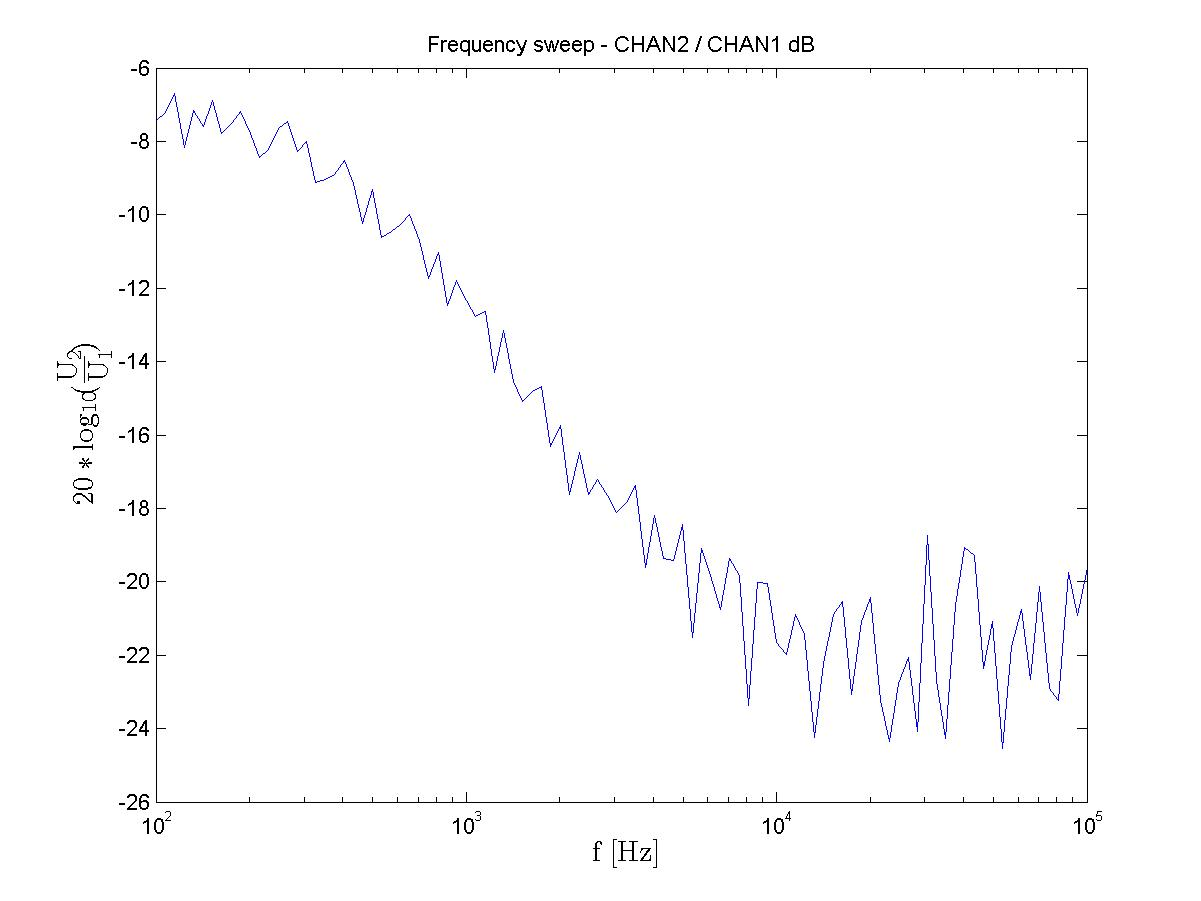
\includegraphics[width=0.8\linewidth]{versuch4/versuch4-100ohm-betrag.jpg}
        \caption{Bode-Diagramm für $R_L=100\si{\ohm}$, Betrag $\underline{U}_2/\underline{U}_1(\omega)$}
        \label{fig:4-100ohm-betrag}
\end{figure}

% \begin{figure}{H}
%     \centering
%     \includegraphics[width=0.8\linewidth]{versuch4/versuch4-100ohm-phase.jpg}
%     \label{fig:4-100ohm-phase}
%     \caption{Bode-Diagramm für $R_L=100\si{\ohm}$, Phase $\varphi (\omega)$}
% \end{figure}


\begin{figure}[H]
        \centering
        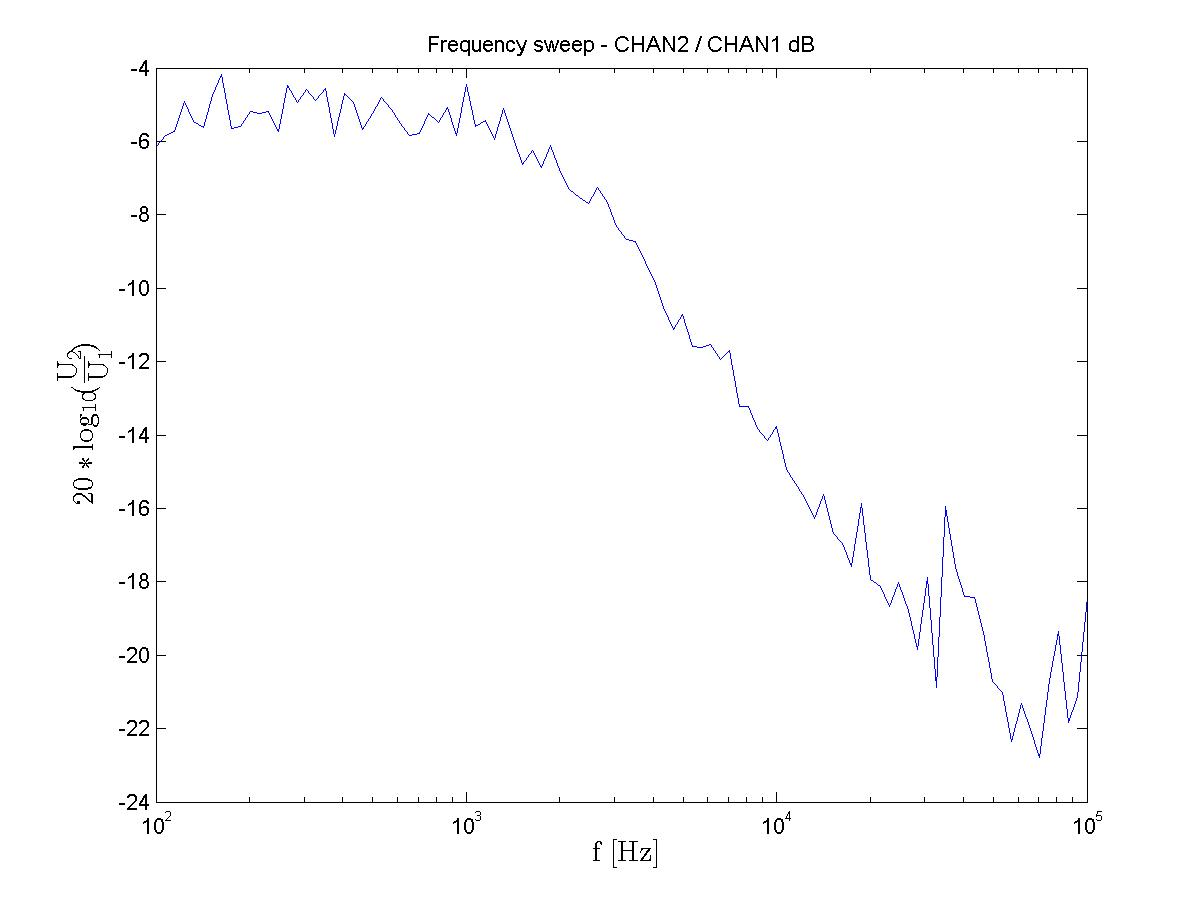
\includegraphics[width=0.8\linewidth]{versuch4/versuch4-680ohm-betrag.jpg}
    \caption{Bode-Diagramm für $R_L=680\si{\ohm}$, Betrag $\underline{U}_2/\underline{U}_1(\omega)$}
    \label{fig:4-680ohm-betrag}
\end{figure}

% \begin{figure}[H]
%     \centering
%     \includegraphics[width=0.8\linewidth]{versuch4/versuch4-680ohm-phase.jpg}
%     \label{fig:4-680ohm-phase}
%     \caption{Bode-Diagramm für $R_L=680\si{\ohm}$, Phase $\varphi (\omega)$}
% \end{figure}


\begin{figure}[H]
    \centering
    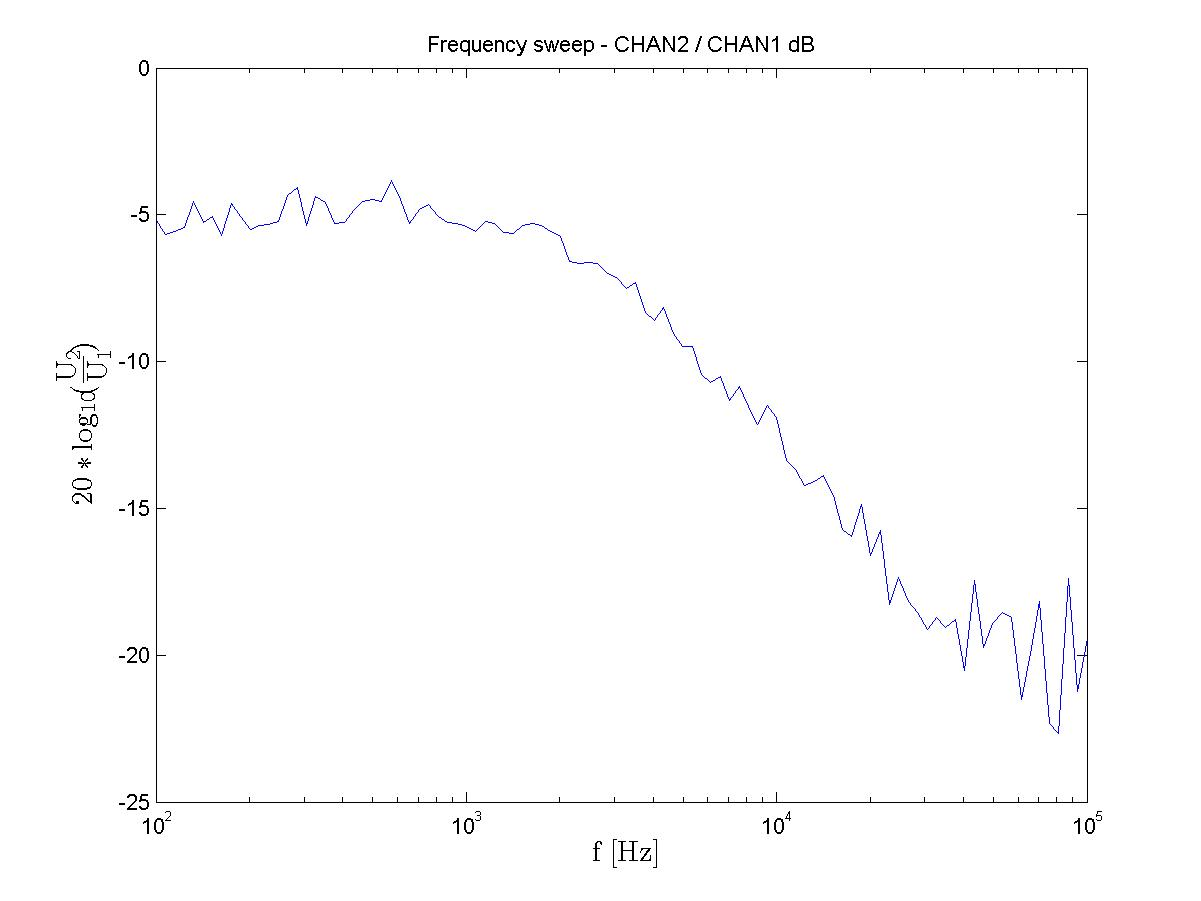
\includegraphics[width=0.8\linewidth]{versuch4/versuch4-1kohm-betrag.jpg}
    \caption{Bode-Diagramm für $R_L=1\si{k\ohm}$, Betrag $\underline{U}_2/\underline{U}_1(\omega)$}
    \label{fig:4-1kohm-betrag}
\end{figure}

% \begin{figure}[]H]
%     \centering
%     \includegraphics[width=0.8\linewidth]{versuch4/versuch4-1kohm-phase.jpg}
%     \label{fig:4-1kohm-phase}
%     \caption{Bode-Diagramm für $R_L=1\si{k\ohm}$, Phase $\varphi (\omega)$}
% \end{figure}


\end{document}